\documentclass{LULCSProject}
\usepackage{amsmath}
\usepackage{enumitem}
\usepackage{listings, listings-rust}
\usepackage{graphicx}
\usepackage{todonotes}
\usepackage{hyperref}

\newcommand{\tvect}[3] { \ensuremath{\Bigl(\negthinspace\begin{smallmatrix}#1\\#2\\#3\end{smallmatrix}\Bigr)}}
\newcommand{\twovect}[2] { \ensuremath{\left(\negthinspace\begin{smallmatrix}#1\\#2\end{smallmatrix}\right)}}

\title{An Open Source Smart home Platform}
\author{Niklas Harnish}
\date{12/05/2023}
%\BSc % \MEng \BEng etc. 
\supervisor{Dr Amna Asif}

\wordcount{0} % number of words in your report 


\abstract{Put your abstract here. You should create a short abstract (200
words at maximum) which is on a page by itself. The abstract should be
a very high-level overview: for example 1--2 sentences on the aims of
the project, 1--2 sentences on the kind of design, implementation, or
empirical work undertaken, and 2--3 sentences summarising the primary
contribution or findings from your work. The abstract appears in the
front matter of the report: after your title page but before the table
of contents.

what should go in here:
\list{}
    \item aims
    \item design
    \item implementation
    \item findings and primary contribution

}


\declaration{
  Put some text similar to the following in here:\\[.5em]
I certify that the material contained in this dissertation is my own work and does not contain
unreferenced or unacknowledged material. I also warrant that the above statement applies to the
implementation of the project and all associated documentation. Regarding the electronically
submitted work, I consent to this being stored electronically and copied for assessment purposes,
including the School's use of plagiarism detection systems in order to check the integrity of
assessed work.\\
I agree to my dissertation being placed in the public domain, with my name explicitly included
as the author of the work.\\
Name:\\
Date:
}

\dedication{
  If you want to dedicate to someone in particular
}

\acknowledgements{
  General acknowledgements \ldots

  your supervisor, your family, your
  friends, \ldots
}

\begin{document}

\maketitle

\pagenumbering{Roman}

%\tableofcontents

\listoffigures
\newpage
% \begingroup
% \let\clearpage\relax
\listoftables
%\endgroup

\newpage
\pagenumbering{arabic}

%%
%% include your chapters here
%%
\chapter{Introduction} \label{cha:intro}
\todo{actually write this section}Will write a couple of words about the project 
here, similar projects, inspirations etc. Citation here to remember how to do it 
:)

\section{Aims \& Objectives} \label{sec:intro:aims}
When researching available smart home technology, one major gap I came across 
was the availability of open source software. While options exist for someone 
interested in connecting their proprietary device to an open source platform 
(view \todo{find the link to this}), there was no solution for anyone looking to 
build their own device and then connect it to an open source hub. In fulfilling 
this goal, to build an open source platform for both devices and the hub they 
will connect to, there are multiple objectives that will need to be met along 
the way:
\begin{enumerate}
    \item Create a Library and API (Application Programming Interface) for 
        building smart home devices.
    \item Build a Server with an API for the smart home devices to communicate 
        with. This will act as a hub and will control clients connected to it.
         \begin{enumerate}
             \item This API should be well documented, so a user can interact 
                 with the hub, without using the Library.
         \end{enumerate}
     \item Create a frontend, which will be populated with devices currently 
         connected to the smart home. It will also be used to control clients 
         connected to the server.
         \begin{enumerate}
             \item The API provided by the server for this frontend should also 
                 be easy to use, so the user can create their own frontend 
                 environment.
         \end{enumerate}
     \item The code of all of the above should be hosted in a public repository, 
         with instructions for how to build and use every component of the 
         system.
         \begin{enumerate}
             \item An appropriate license should also be selected for this 
                 repository, so the code within it can be copied or modified by 
                 third parties.
             \item This repository should provide important links and provide 
                 information on the inner workings of the system, to support 
                 interested parties.
         \end{enumerate}
\end{enumerate}
    
\section{Project Overview} \label{sec:intro:overview} \todo{ask about this 
section}
\textit{Each bullet point below would give a small summary of the section}
\begin{enumerate}
    \item \textbf{Background Research} 
    \item \textbf{Design of the System \& Technology Decisions}
    \item \textbf{Implementation}
    \item \textbf{Results}
    \item \textbf{Conclusion and Reflection}
chapter1.tex
\end{enumerate}


% Always start your chapter on a new page!
\newpage
\chapter{Background} \label{cha:chapter2}

\section{IoT System Architectures} \label{sec:chap2:architectures}
Kamienski et al. describe a simple three layer architecture of an IoT system in \cite{DesigningOpenIotSystem}. Within this architecture, the top layer is the "Input System", from which any data that will influence the decisions of the IoT system will come from. Included in this are sensors, but also user facing interfaces. The second layer, known as the "Process System", is where any algorithms are run and system behavioral decisions are made. The goal of this layer is to gain an "improved understanding of the system where the  data comes from" \cite{DesigningOpenIotSystem}. The bottom layer is the "Output System", which are where decisions made by the Process System will be enacted. This is often represented as the devices connected to the IoT system.

This three layer architecture is expanded upon by Bansal and Kumar within \cite{IotEcosystemSurvey}, where three more architectures are described which expand upon the ideas within the three layer architecture. They are however more specialized than the three layer architecture. The first of these is a "Middleware Based" architecture, which can take many forms, but is usually combined with another type of architecture, with a middleware layer. The different types are described in detail by Zhang et al. in \cite{MiddlewareIOTSurvey}. The second is known as a "Fog Based" architecture, where certain tasks, usually those with less processing requirements, are calculated on device to reduce latency. More computationally expensive tasks are however calculated on a server in the cloud \cite{IoTArchitectures}.

The most relevant architecture to this report is known as a "Service Based" architecture (SBA). The SBA is defined around the concept of the Service Oriented Architectural (SOA) style \cite{InteractingSoaBasedIot} of software design. SOA is defined by the Open Group Foundation as an "architectural style that supports service-orientation", where a service is a "logical representation of a repeatable business activity that has a specified outcome" \cite{SoaSourceBook}. Each service is a "black box" any device interacting with it. Other devices use interfaces and API endpoints to make requests to the service and receive a result. A SOA is comprised of many different services. In SBA, services are used to offer device functionality using interfaces, often using web based concepts such as SOAP or REST APIs \cite{TrustManagementSoaIot}. This allows devices with different capabilities and purposes to interact with the same system, allowing for an IoT system that is more flexible. 


\section{The Smart Home System} \label{sec:chap2:smarthome}
Sethi and Sarangi define six components that need to be present within a social IoT setting. A social IoT system is defined as a IoT system where devices form relationships with other devices. While our smart home system will not be a social IoT system, some of these concepts are still of interest. These are: \todo{ask if this is ok with citation as its quite similar}
\begin{enumerate}
    \item ID: the device within the system needs to have a way of identifying 
        it.
    \item Meta-data: the device should have information regarding its form and 
        purpose
    \item Security Controls: the system should have some way of distinguishing 
        between different users. It should also be able to distinguish what 
        types of devices it can connect to or can connect to it.
    \item Service Discovery: each device should be able to discover other 
        devices connected to the system and what services they offer.
\end{enumerate}

There are some specific constraints specific to Smart Homes. Reliability is a key concern, due to the lack of a trained professional being available to fix any issues that arise. This is contrast to more industrial IoT settings, where there might be someone to fix any issues that arise. Another concern is the security and privacy of the system. Due to smart homes inherently having access to sensitive data (due to their position in someone's home), one must ensure that the system is both ethically sound and secure. The issue of security is further discussed in Subsection~\ref{sec:chap2:security}.
\todo{further add to this section, just not sure what yet}

\section{APIs and Web Interfaces} \label{sec:chap2:frontend}
\section{Security} \label{sec:chap2:security}
\section{Networking} \label{sec:chap2:networking}
\section{Open Source and Licensing} \label{sec:chap2:opensource}



\newpage
\chapter{Implementation} \label{cha:chapter3}

\section{Technology Choices} \label{sec:chap3:technology}
This section will discuss choices that have been made throughout the project regarding technology used and justifications for their usage.

\subsection{Rust} \label{sec:chap3:technology:rust}
There were a few requirements when choosing an appropriate programming language for this project:
\begin{enumerate} 
    \item Performance: There are two aspects to performance within this project. Performance considerations and optimization are vital on IOT devices themselves, due to their limited on-board processing power. On the other hand, while performance on servers is definitely important, it is significantly easier to scale server-performance, by simply adding more servers (horizontal scaling) or by improving the hardware of any individual server (vertical scaling), than it is to improve performance of an IoT device. This is especially true of an IoT device that is already deployed.
    \item Stability: Another important requirement when choosing a language is the stability of code written in the language. This does not necessarily mean that code written in any language is inherently unstable. This requirement is more of a consideration about if a language enables and encourages a programmer to write code that is memory-safe and handles errors correctly. This is important in an IoT environment, as devices are expected to run for long periods. What is the point of a security camera if it's software crashes every couple days, due to an obscure memory out of bounds error? 
    \item Security: While no language is inherently "hack-proof" or secure, there are ways a language can encourage behaviors that can lead to better outcomes in security. A blog-post by the "Microsoft Security Response Centre" states that 70\% of all vulnerabilities assigned a CVE (Common Vulnerabilities and Exposures) each year are due to memory corruption errors \cite{ProactiveApproachToSecureCode}. In the post the languages "C" and "C++" are specifically referred to as being part of this problem. As mentioned in subsection ~\ref{sec:chap2:security}, security is of particular importance in smart home systems, so ensuring a method or language that enables secure code is chosen is of particular importance. 
    \item Ease of Use and Comfort: While not particularly important in the final product, having a language that is easy to develop in can make the developer experience easier and can lead to faster iteration on ideas, perhaps leading to a better final result. That being said, developer familiarity with a language can more than make up this difference. A seasoned C++ developer will be able to iterate faster and produce a better product in C++, than if they are using an "easy" language, that they are not as familiar with.
\end{enumerate}\todo{not sure I like the list style here}
After some deliberation, the language that was chosen for this project was Rust. While C/C++'s performance rivals and often surpasses Rust, the difference is often quite marginal \cite{PerformanceEvalOnMicrocontroller}, due to all three being compiled to machine code. What makes Rust different, is its headline feature, known as the "borrow checker". While the details of the borrow checker are out of scope of this paper, it can ensure that at compile-time, the code is memory safe. While there are ways to circumvent this (using the "unsafe" keyword), this has to be explicitly done. Due to the code being guaranteed memory safe at compile time, outside the aforementioned unsafe blocks, Rust code is known for its ability to run long-term without running into crashes. Additionally, Rust code is a popular choice for embedded devices, due to being able to compile without a standard library (this has to be enabled), giving it flexibility in a project such as this.

I have decided to use Rust for both the Server and Clients. While Rust might be a somewhat obvious choice for IoT clients, it is less so for servers. Due to the "borrow checker", while Rust might be safe, it is often said to be harder to write than traditional languages. This makes it more questionable as the primary language for the server, due to it being a less constrained platform (view performance section above). While servers are theoretically almost infinitely horizontally scalable, in practice this is often not the case, especially in a smart-home's case, as they have to fit in someone's home and generally should be affordable. Therefore, ensuring that the server can run on as many devices as possible, be it a Raspberry-Pi, or a modern desktop, is an important goal to strive for. The "difficulty" aspect of Rust can be largely counteracted by personal familiarity with the language. Additionally, having a stable server is very important, especially since all IoT devices will need to frequently communicate with this server, an aspect which Rust excels at. Rust also has a thriving community of libraries (known as crates), which using the language gives access to. For these reasons I have chosen Rust as the primary programming language of the Server and Client parts of this project.

\subsection{gRPC} \label{sec:chap3:technology:grpc}
gRPC is an RPC implementation released by Google in 2015. It uses Protocol Buffers (protobufs) as an interface definition language (IDL), to define services on servers, that clients can then call, such as any RPC library. The server runs a gRPC server and the client runs the gRPC client \cite{grpcHomepage}. Protobufs are compiled to many different languages, with many different libraries available for these languages, that automate much of the process. In a performance comparison between REST, gRPC, websockets, GraphQL, gRPC came out ahead in many different metrics \cite{reviewOfInternetProtocols}. These include: 
\begin{itemize}
    \item inserting one value into a database
    \item fetching one value from a database 
    \item fetching one hundred elements  
\end{itemize}
in both native and containerized tests. In fact, gRPC was the most performant internet communication protocol in all metrics apart from memory usage.

Due to its performance and cross-language support I have chosen gRPC as the internet communication protocol for this project. The specific library used for this project is known as "Tonic". Tonic is a Rust gRPC crate that includes both a gRPC server and client. It also utilizes "prost" to compile protobuf files into Rust code, without having to interface the protobuf compiler itself. All protobuf files are compiled as a compilation step of the server and client, eliminating the need for external build scripts (this is only partially true, view Sub Section~\ref{sec:chap3:server:protoBufs}).

\subsection{Typescript \& VueJS} \label{sec:chap3:technology:ts}
While a Command Line Interface (CLI) frontend, written in Rust, will be made available, the main focus will be on the Graphical User Interface (GUI). To ensure that it can run on a variety of systems and is relatively easy to create, it will be web based, using Javascript at runtime. However, it will be written in Typescript. Typescript is a superset of Javascript, that compiles to Javascript and leaves no trace of types behind. Typescript provides a robust type-system, including, but not limited to \cite{understandingTypescript}:
\begin{itemize}
    \item Structural type equivalence, instead of Javascript's by-name type equivalence
    \item Types and concepts for object-based programming
    \item Type operators
\end{itemize}
All of these, while not guaranteeing that the program will be type-safe at runtime, help a developer design more robust and long term solutions generally associated with statically typed languages.

In conjunction with Typescript a web-development framework will be used. Web frameworks are libraries for Javascript that allow easier development of websites and web apps, often incorporating HTML (HyperText Markup Language) and CSS (Cascading Style Sheets) code into Javascript code. They also provide reactivity, meaning that if a variable changes in the code, that change can easily be reflected on the site. This can be done in most frameworks by simply using the variable in the HTML code, something that standard HTML does not support (methods of doing this differs between frameworks).

Most of the choice between different web-frameworks comes down to personal preference and familiarity with a framework. That being said there can be performance differences between different frameworks, that could make a difference on some systems. While there is a lack of formal experiments on framework performance, an informal experiment \cite{performanceComparisonJS} showed that while there is a performance difference between different frameworks, it should not be the primary decision maker. When the difference when creating 1000 rows between vanilla JavaScript and VueJS is 32 milliseconds, the disparity will not be noticeable to the end user. For this reason, and personal familiarity with the framework, I have decided to use VueJS as the frontend development framework for this project.

\subsection{Raspberry Pi} \label{sec:chap3:technology:raspi}
\todo{write this}

\section{Server \& Hub} \label{sec:chap3:server}
Due to the server being the largest part of this project, and practically being a requirement for testing the client and frontend functionality, this will be focused on first. This section will describe defining and compiling protobuf files for API endpoints, server startup, how IOT devices are registered, security mechanisms and how concurrency was handled within the server. 

\subsection{Protocol Buffers and Tonic} \label{sec:chap3:server:protoBufs}
Protobufs are defined within ".proto" files. They use a fairly basic syntax, where the user can define a service using the "service" keyword. A service can contain many functions which a client can call, these are defined using the "rpc" keyword. You can also define the arguments this function takes and what it returns. Structs are defined using the "message" keyword, where each field is separated by a semicolon. Fields can have multiple modifiers, including optional, repeated and map. Repeated marks a field as possibly being a list, or array structure. Map marks a field as being a map data structure. Finally, messages from other files can be imported, using the import keyword and then giving the file-name. \cite{protobufDocs} For an example of a protobuf file view \textbf{\textit{protos/iot/registrationService.proto}}:

\begin{lstlisting}[language=protobuf3, style=boxed]{iot/registrationService.proto}
syntax = "proto3";
package iot.registration;
import "types.proto";

service RegistrationService {
    rpc Register(
        RegistrationRequest
    ) returns (RegistrationResponse);
};

message RegistrationRequest {
    string public_key = 1;
    string name = 2;
    repeated iot.types.DeviceCapabilityStatus capabilities = 3;
}

message RegistrationResponse {
    string public_key = 1;
    string client_id = 2;
    string certificate = 3;
}
\end{lstlisting}

Here we define a service called "RegistrationService", with a function called Register. This function is called by IOT clients when they first attempt to connect to the server which takes a RegistrationRequest as a parameter and returns a RegistrationResponse. The file also defines two "messages", the aforementioned RegistrationRequest and RegistrationResponse. While most of the fields within them are fairly obvious, RegistrationRequest.capabilities warrants further explanation.
    This field is repeated, meaning it is an array data structure. This array contains the type DeviceCapabilityStatus, which is defined in iot.types. We can see this type is imported at the top of the file, from "types.proto". This is the definition of DeviceCapabilityStatus:

\begin{lstlisting}[language=protobuf3, style=boxed]{iot/types.proto}
message DeviceCapabilityStatus {
    bool available = 1;
    string capability = 2;
}
\end{lstlisting}

In summary, if an IOT device wants to register with this server, they will need to call the Register server stub. The server stub takes one parameter, the RegistrationRequest message. This message requires the client to give it's public key, it's display name and an array of "DeviceCapabilityStatus". The Register function then returns a RegistrationResponse. 

To compile these server stubs to Rust we will be using the aforementioned Rust "Tonic" crate. To do this first we must add the "Tonic" crate to our project, then add "tonic-build" to our build dependencies (view Cargo Documentation). We then create a build.rs file, which is run when the Rust compiler (Cargo) builds the program. You can view the file \textbf{\textit{backend/build.rs}} below:

\begin{lstlisting}[language=Rust, style=boxed, showstringspaces=false]{backend/build.rs}
fn main() -> Result<(), Box<dyn std::error::Error>> {
    tonic_build::compile_protos(
        "../proto/iot/types.proto"
    )?;
    tonic_build::compile_protos(
        "../proto/iot/registrationService.proto"
    )?;
    tonic_build::compile_protos(
        "../proto/iot/requestUpdateService.proto"
    )?;
    tonic_build::compile_protos(
        "../proto/iot/deviceControlService.proto"
    )?;

    tonic_build::configure()
        .type_attribute(
            ".", 
            "#[derive(serde::Deserialize, serde::Serialize)]"
        )
        .compile(
            &[
                "../proto/frontend/registrationService.proto",
                "../proto/frontend/frontendTypes.proto",
                "../proto/iot/types.proto",
                "../proto/frontend/deviceControlService.proto",
            ],
            &["../proto/frontend", "../proto/iot"],
        )?;
    Ok(())
}
\end{lstlisting}

In line 2-13 we are telling tonic\_build, using prost under the hood (which in turn calls the protobuf compiler), to compile the files required for Device \& Server communication. We do this by calling the \textit{compile\_protos} function. The files in the folder \textit{proto/iot} are the ones used by IOT devices. This is quite simple to use, however is technically a build script, making the statement in subsection~\ref{sec:chap3:technology:grpc} partially untrue. Line 15-28 are where frontend protobuf files are compiled. These require the traits (Rust equivalent to interfaces in other languages) "Serialize" and "Deserialize" to be implemented for all structs compiled from the files. We therefore require this special syntax when compiling them. For more information on why they need these traits, view subsection~\ref{sec:chap3:frontend:json}.

Finally, protobuf server-stubs and messages can be imported into Rust using a macro provided by tonic. View below how \textbf{\textit{backend/src/server/registration.rs}} imports the \textit{protos/iot/registration.proto} file:

\begin{lstlisting}[language=Rust, style=boxed]{server/registration.rs}
use crate::types::types;
pub mod registration_service {
    tonic::include_proto!("iot.registration");
}
\end{lstlisting}

In order to import the compiled protbuf file, we simply call the "include\_proto" macro (it being a macro is indicated by the \textbf{!}). Note that we need to import the types module first, as this module contains the compiled \textit{protos/iot/types.proto} file, which is imported by \textit{registration.proto}. Additionally, instead of giving the file path to the protobuf file, we simply give the module name, which is also defined in the protobuf file.

\subsection{Server Start Up} \label{sec:chap3:server:startup}
\todo{maybe add a section on how cli arguments are parsed if i need more words (probably not)}

This subsection details what the server handles at startup, including starting the GRPC server, creating server stubs and creating a JSON web server (again, for an explanation on why this is necessary view subsection~\ref{sec:chap3:frontend:json}). Below you can see how I instantiate a new gRPC server instance within \textbf{\textit{backend/src/server/server.rs}}:

\begin{lstlisting}[language=Rust, style=boxed, showstringspaces=false]{}
let grpc_server = tonic::transport::Server::builder()
    .add_service(
        registration_service_server
            ::RegistrationServiceServer::new(
                registration_service,
        )
    )
    .add_service(
        request_update_service_server
            ::RequestUpdateServiceServer::new(
                polling_service,
        )
    )
    .add_service(
        frontend_registration_service_server
            ::FrontendRegistrationServiceServer::new(
                frontend_registration_service,
        ),
    )
    .add_service(
        frontend_device_control_service_server
            ::FrontendDeviceControlServiceServer::new(
                device_control_service,
        ),
    )
    .serve_with_shutdown(
        grpc_address,
        tokio::signal::ctrl_c().map(drop)
    );

println!("Started GRPC Server on {}", grpc_address);

let grpc_handle = tokio::spawn(async move { grpc_server.await });
\end{lstlisting}

The Server struct comes from the tonic crate and transport module. We invoke the builder method on the Server struct, a very common pattern within the Rust ecosystem. In fact, the same pattern is used instantiate a new IoT device in the client library (view section~\ref{sec:chap3:devicelib}). After invoking the builder method, which returns a new Server struct, we add services to it. A service is simply an instance of a struct which implements a trait (interface) generated by the protobufs. For an example of this, view subsection~\ref{sec:chap3:server:registration}. These are created above the code snippet.

The "server\_with\_shutdown" method consumes the Server struct and runs the server, on the address handed to it in the parameter. In this case it is the variable "grpc\_address", which is a string containg the device's IP address and the user specified port. The second parameter simply tells Rust to drop the gRPC server (shutdown and gracefully free the memory associated with it) when the key combination crtl-c is pressed. This is an easy way to implement this behavior in Rust when working with multiple threads (view subsection~\ref{sec:chap3:server:threads}).

Once we have added all services to the Server struct. We can then "await" the gRPC server handle on another thread. For more information on how this works, view subsection~\ref{sec:chap3:server:threads}.  

The JSON HTTP server (view ~\ref{sec:chap3:frontend:json}) works almost the same, using the same builder pattern. View part of the "run\_json\_frontend" function, found in the file \textbf{\textit{backend/src/server/server.rs}} below:
\begin{lstlisting}[language=Rust, style=boxed, showstringspaces=false]{}
    let result = actix_web::HttpServer::new(move || {
        let cors = actix_cors::Cors::permissive();
        App::new()
            .app_data(web::Data::new(json_state.clone()))
            .wrap(cors)
            .service(json_registration::json_registration)
            .service(json_registration::json_registration_options)
            .service(json_get_devices::json_get_connected_devices)
            .service(json_get_devices
                ::json_get_connected_devices_options
            )
            .service(json_device_control::json_device_control)
            .service(json_device_control
                ::json_device_control_options
            )
    })
    .bind(JSON_ADDRESS)?
    .run();

    println!("Successfully Started JSON API Layer on {JSON_ADDRESS}");
\end{lstlisting}
Due to this builder function requiring more Rust specific knowledge to understand, it will be simplified here. It is functionally the same as the one seen from Tonic. To host this HTTP server we are using the popular crate named "Actix", a self described "powerful, pragmatic, and extremely fast web framework for Rust" \cite{actixWebsite}.
\subsection{Device Registration} \label{sec:chap3:server:registration} 


\subsection{Security} \label{sec:chap3:server:security}

\subsection{Threads \& Concurrency} \label{sec:chap3:server:threads}


\section{Device Library} \label{sec:chap3:devicelib}
\section{Example Device} \label{sec:chap3:deviceexample}
\section{Networking}

\section{Web \& CLI Frontend} \label{sec:chap3:frontend}
\subsection{Using JSON for the Frontend API} \label{sec:chap3:frontend:json}
\section{Open Source} \label{sec:chap3:opensource}


%%
%% You bib file
%%
\newpage
\bibliography{report}
\todo{ask about SOA source book citation}

\newpage
\appendix
%%
%% Your appendices
%%
\chapter{Original Project Proposal}
\label{chap:A1}

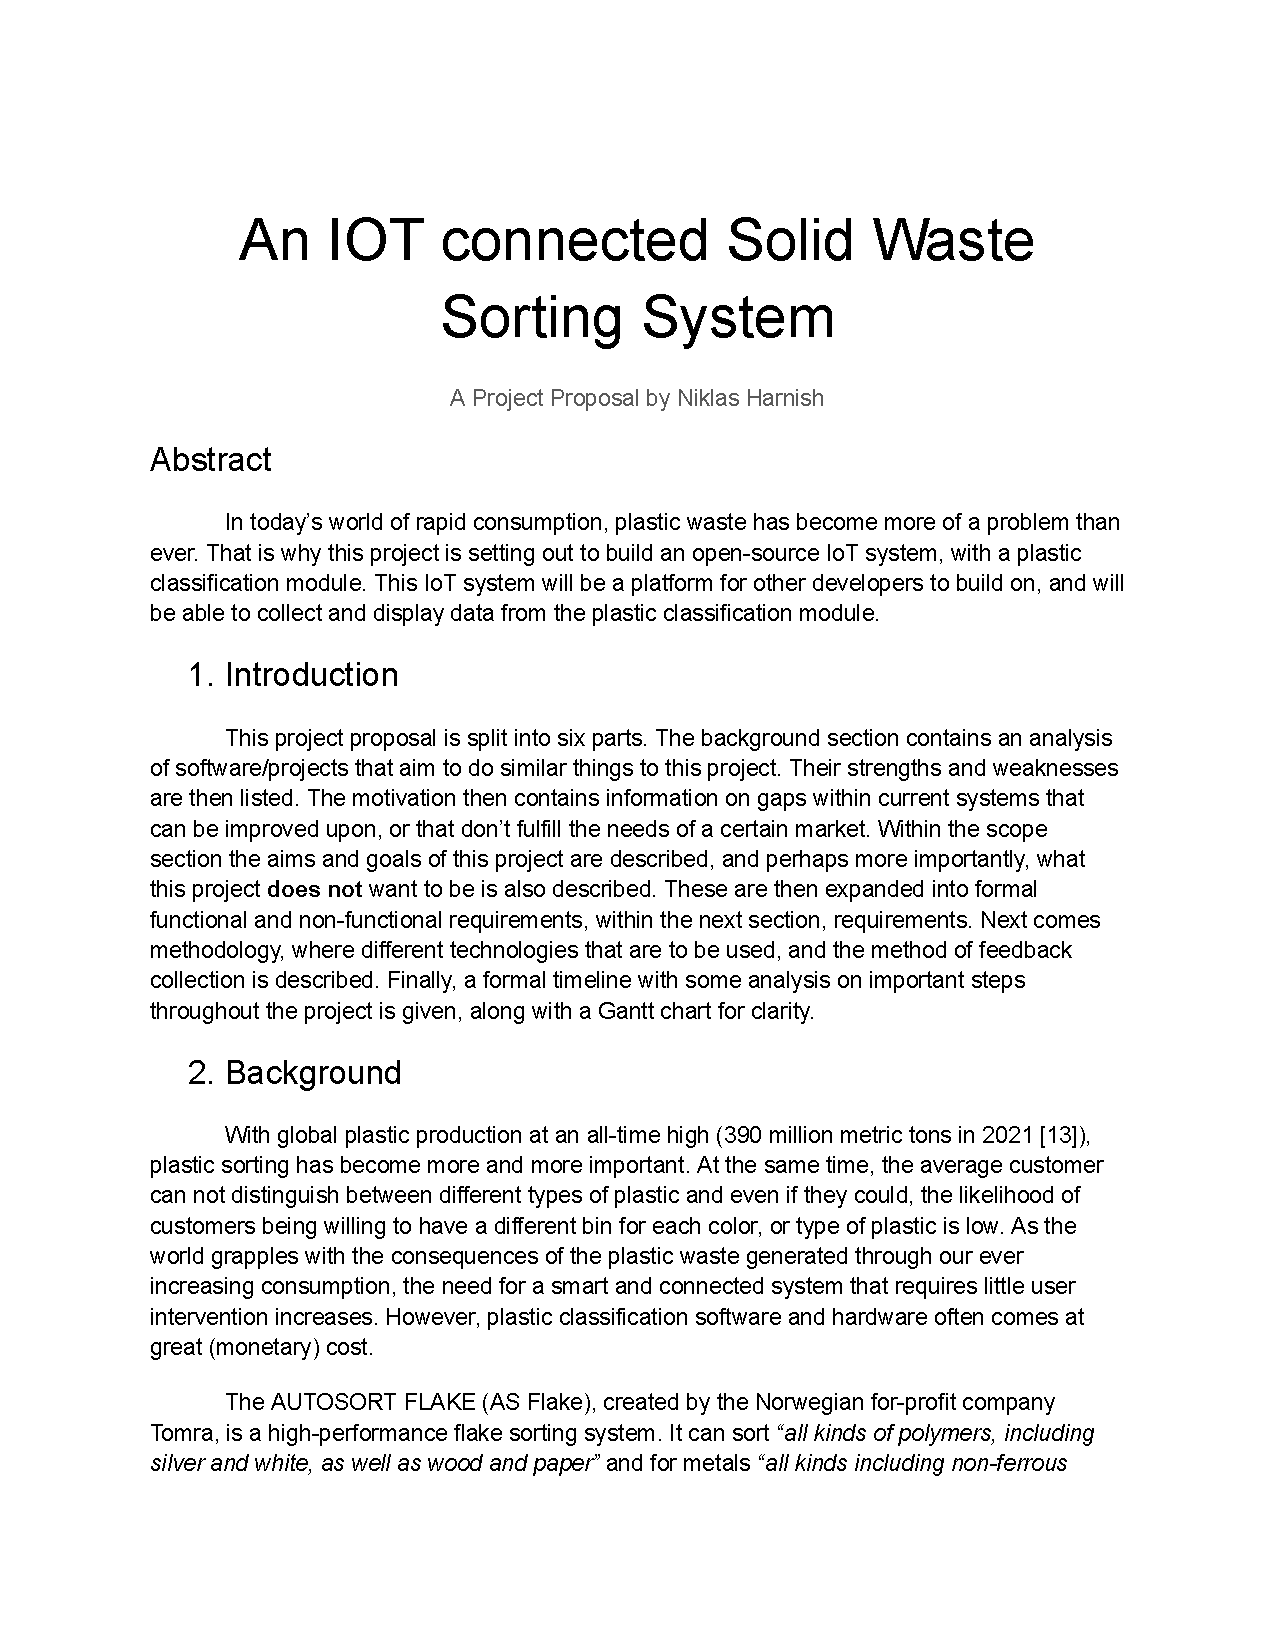
\includepdf[pages=-]{project_proposal.pdf}

\newpage

\chapter{Another Appendix Chapter}
\label{chap:A2}

This could be about your experiments

\end{document}
